%%%%%%%% ICML 2019 submission %%%%%%%%%%%%%%%%%

\documentclass{article}

\usepackage{icml2019}
% \usepackage[accepted]{icml2019}

\usepackage{microtype}
\usepackage{graphicx}
\usepackage{subfigure}
\usepackage{booktabs}
\usepackage{hyperref}
\usepackage{amsmath}
\usepackage{amsfonts, amsthm, amssymb}
\usepackage{graphicx}
\usepackage[parfill]{parskip}
\usepackage{enumerate}
\usepackage[shortlabels]{enumitem}
\usepackage{bm}

\newcommand{\diam}{\mathrm{diam}}
\newcommand{\set}[1]{\left\{#1\right\}}
\newcommand{\defeq}{\overset{\mathrm{def}}{=}}
\newcommand{\vol}{\mathrm{vol}}
\newcommand{\cut}{\mathrm{cut}}
\newcommand{\abs}[1]{\left \lvert #1 \right \rvert}
\newcommand{\N}{\mathbb{N}}
\newcommand{\Reals}{\mathbb{R}}
\newcommand{\Rd}{\Reals^d}
\newcommand{\norm}[1]{\left\lVert#1\right\rVert}
\newcommand{\1}{\mathbf{1}}
\newcommand{\Phibf}{\mathbf{\Phi}}
\newcommand{\Psibf}{\mathbf{\Psi}}
\newcommand{\dist}{\mathrm{dist}}

%%% Vectors
\newcommand{\pbf}{\mathbf{p}}
\newcommand{\qbf}{\mathbf{q}}
\newcommand{\ebf}[1]{\mathbf{e}_{#1}}
\newcommand{\pibf}{\bm{\pi}}

%%% Matrices
\newcommand{\Abf}{\mathbf{A}}
\newcommand{\Xbf}{\mathbf{X}}
\newcommand{\Wbf}{\mathbf{W}}
\newcommand{\Lbf}{\mathbf{L}}
\newcommand{\Dbf}{\mathbf{D}}
\newcommand{\Ibf}[1]{\mathbf{I}_{#1}}

%%% Probability distributions (and related items)
\newcommand{\Pbb}{\mathbb{P}}
\newcommand{\Cbb}{\mathbb{C}}

%%% Sets
\newcommand{\Cset}{\mathcal{C}}
\newcommand{\Aset}{\mathcal{A}}
\newcommand{\Asig}{\Aset_{\sigma}}
\newcommand{\Csig}{\Cset_{\sigma}}

%%% Operators
\DeclareMathOperator*{\argmin}{arg\,min}


%%% Algorithm notation
\newcommand{\ppr}{{\sc PPR}}
\newcommand{\pprspace}{{\sc PPR~}}

\newtheoremstyle{aldenthm}
{6pt} % Space above
{6pt} % Space below
{\itshape} % Body font
{} % Indent amount
{\bfseries} % Theorem head font
{.} % Punctuation after theorem head
{.5em} % Space after theorem head
{} % Theorem head spec (can be left empty, meaning `normal')

\theoremstyle{aldenthm}
\newtheorem{theorem}{Theorem}
\newtheorem{definition}{Definition}
\newtheorem{lemma}{Lemma}
\newtheorem{corollary}{Corollary}

\newtheoremstyle{aldenrmrk}
{6pt} % Space above
{6pt} % Space below
{} % Body font
{} % Indent amount
{\itshape} % Theorem head font
{.} % Punctuation after theorem head
{.5em} % Space after theorem head
{} % Theorem head spec (can be left empty, meaning `normal')

\theoremstyle{aldenrmrk}
\newtheorem{remark}{Remark}





\newcommand{\theHalgorithm}{\arabic{algorithm}}


\icmltitlerunning{Local clustering of density upper level sets}

\begin{document}

\twocolumn[
\icmltitle{Local Spectral Clustering of Density Upper Level Sets}

\icmlsetsymbol{equal}{*}

\begin{icmlauthorlist}
\icmlauthor{Alden Green}{cmu}
\icmlauthor{Sivaraman Balakrishnan}{cmu}
\icmlauthor{Ryan Tibshirani}{cmu}
\end{icmlauthorlist}

\icmlaffiliation{cmu}{Department of Statistics and Data Science, Carnegie Mellon University, Pittsburgh PA, USA}

\icmlcorrespondingauthor{Alden Green}{ajgreen@andrew.cmu.edu}

\icmlkeywords{local clustering}

\vskip 0.3in
]

\printAffiliationsAndNotice{}

\section{Empirical Performance of PPR on Gaussian Mixture Models}

The assumptions and theory of Section \textcolor{red}{2} are tailored towards density functions with sharp transitions in gradient around the perimeter of the density cluster. These type of functions will satisfy \textcolor{red}{A3} with a small ratio of $\Lambda_{\sigma}$ to $\lambda_{\sigma}$, while still satisfying \textcolor{red}{A4}, potentially for $\gamma << 1$. 

As mentioned previously, one line of work on spectral algorithms assesses their performance on mixture models. Particularly well-developed is the characterization of clustering performance on Gaussian Mixture Models (GMMs). Gaussian Mixture Models have smooth derivatives, and are therefore not good candidates for our work (at least, for reasonable values of the parameters in \textcolor{red}{(A1)-(A4)} ). Since they are a classical choice in the clustering literature, we investigate \pprspace performance on them empirically.

\begin{figure*}[ht]
	\vskip 0.2in
	\begin{center}
	\centerline{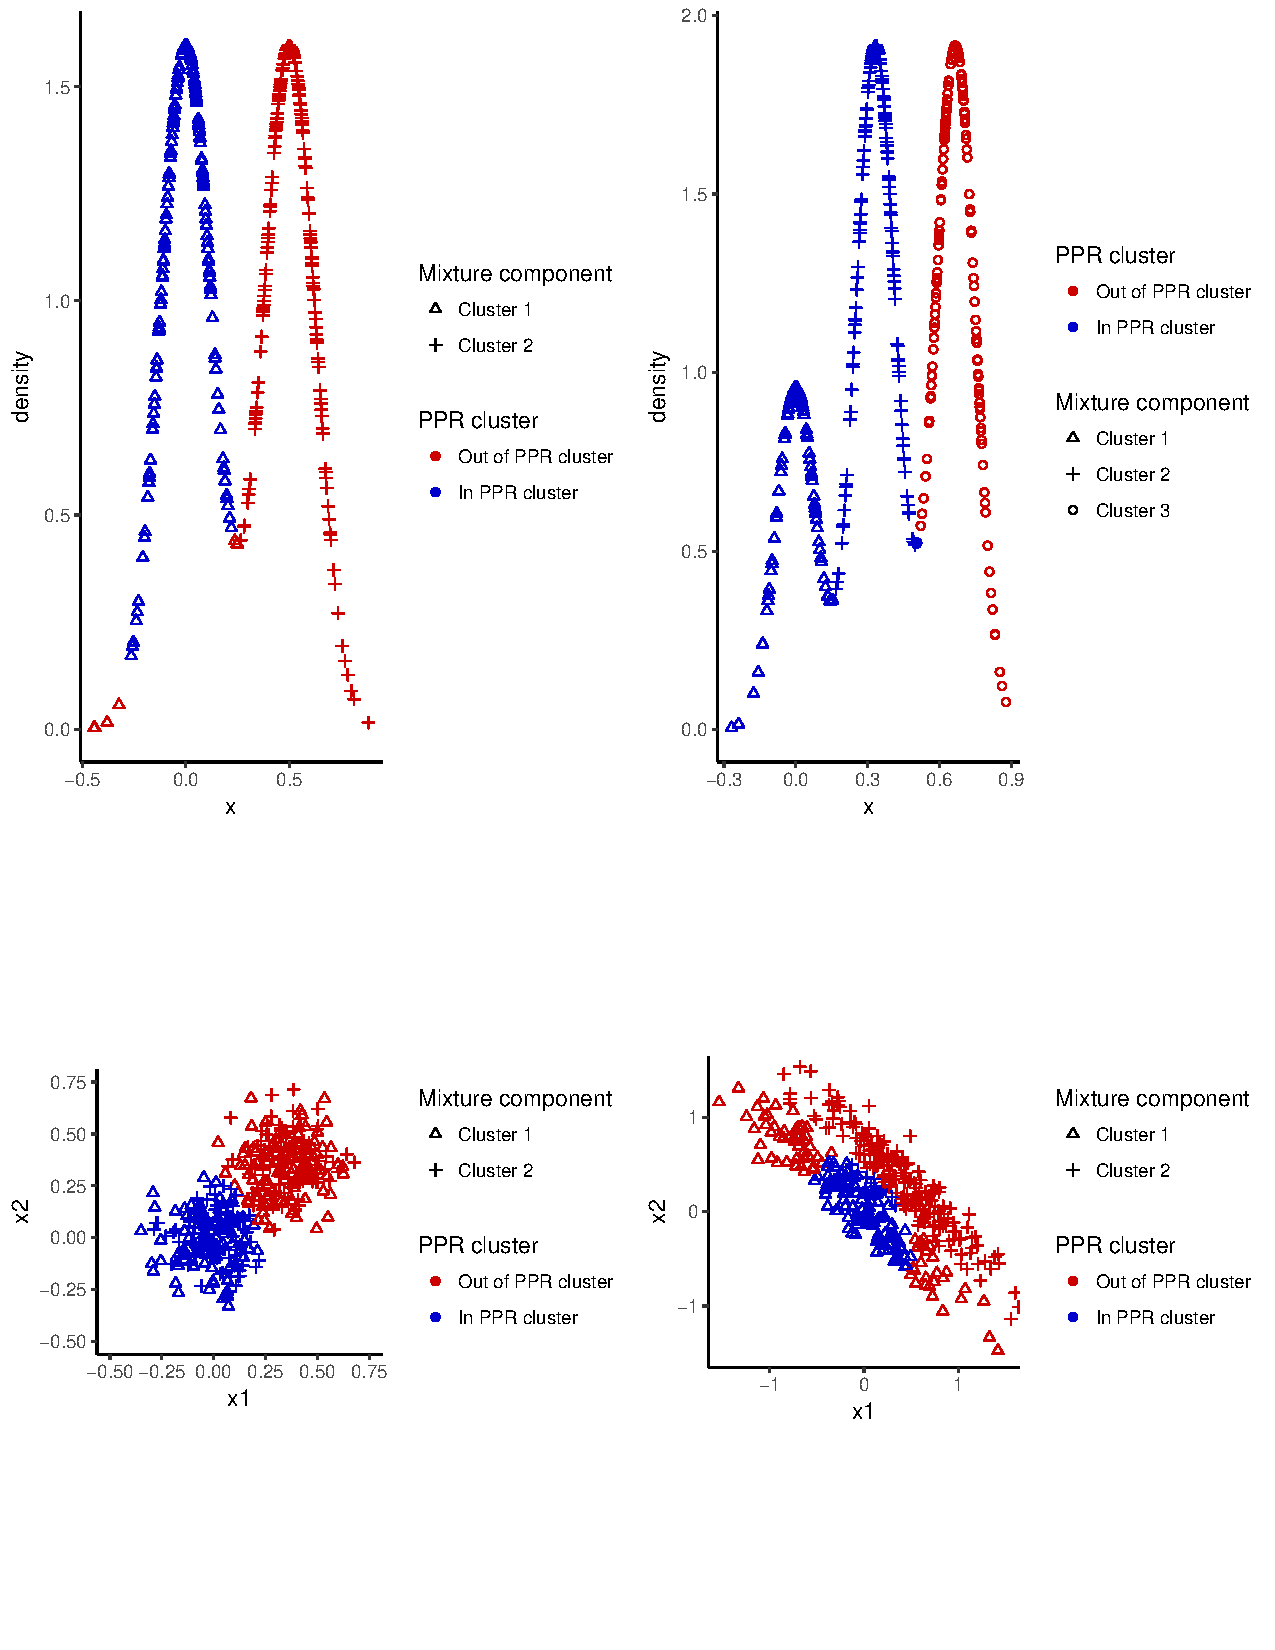
\includegraphics[width=\columnwidth]{graphic_1}}
	\caption{Algorithm \ref{alg: ppr} run over 4 example datasets. Parameters $\alpha$ and $\pi_0$ were tuned to minimize normalized cut of output set. Colors represent \pprspace cuts; shapes correspond to the maximum density among mixture components. Sample size $n = 400$.}
	\label{fig: graphic_1}
	\end{center}
	\vskip 0.2in
\end{figure*}

Figure \ref{fig: graphic_1} tells a story with roughly the same narrative as our theoretical work. The left two plots demonstrate instances, in one and two-dimensions, respectively, where the \pprspace cut has small error relative to a density cut. The right two plots, by contrast, show \pprspace failing to recover, even approximately, a density cut. 

In the bottom right panel in particular, we see the effect of a high diameter on the performance of \pprspace. Although any one vertex on the boundary of a density level set may have few cut edges, the length of the boundary is sufficiently long to make the entire cut too large for \pprspace to select it. Instead, the \pprspace cut defaults to a more geometrically compact shape, which has much smaller (unweighted) perimeter. 

\end{document}